\documentclass{article}
\usepackage[utf8]{inputenc}
\usepackage{amsmath}
\usepackage{amssymb}
\usepackage{graphicx}
\usepackage[a4paper, total={6in, 8in}]{geometry}

\title{Proposta de Abordagem ao Problema do Trabalho Balanceado}
\author{Gustavo Delazeri}
\date{29 de Julho de 2020}

\begin{document}

\maketitle

\section{Formulação do Problema como Programa Inteiro}
\textbf{Variáveis:} 
\begin{itemize}
  \item $x_{ij} \in \{0, 1\}, \quad \forall i,j  \, \mid  \, i \in [n] \land j \in [m]$, onde
  	$$x_{ij} = 
	\begin{cases}
	1,  \quad  \text{Caso tarefa i e executada pelo operador j } \\
	0,  \quad  \text{Caso contrario}
	\end{cases}
	$$
  \item $w_{ijk} \in \{0, 1\}, \quad \forall i,j,k  \, \mid \,  i,j \in [n]  \land k \in [m] \land i \neq j$, onde
  	$$w_{ijk} = 
	\begin{cases}
	1,  \quad  \text{Caso } \,  x_{ik} \land x_{jk} \, \text{é verdade }\\
	0,  \quad  \text{Caso contrario}
	\end{cases}
	$$
	
  \item $y \in \mathbb{R}$, onde
  	$$y = \text{max}\Bigg(\sum_{i \in [n] }^{} p_{ij} \cdot x_{ij},   \forall j \in [m] \Bigg)	$$
\end{itemize}
\textbf{Função Objetivo:} 
	$$\text{Min.} \quad y$$
\textbf{Restrições:} 

\begin{equation}
 	\sum_{j \in [m] }^{} x_{ij} = 1,   \quad \forall i \in [n] 
\end{equation}

\begin{equation}
 	\sum_{i \in [n] }^{} x_{ij}  \geq 1,  \quad  \forall j \in [m] 
\end{equation}

\begin{equation}
 	w_{ijk} \leq (x_{ik} + x_{jk})/2, \quad \forall i,j,k \, \mid \, i,j \in [n]  \land k \in [m] \land i < j
\end{equation}

\begin{equation}
 	w_{ijk} \geq x_{ik} + x_{jk} - 1,  \quad \forall i,j,k \, \mid \, i,j \in [n]  \land k \in [m] \land i < j
\end{equation}

\begin{equation}
 	w_{ijk} \leq x_{j-1k},  \quad \forall i,j,k \, \mid \, i,j \in [n]  \land k \in [m] \land i < j
\end{equation}

\begin{equation}
 	y \geq \sum_{i \in [n] }^{} p_{ij} \cdot x_{ij},   \quad \forall j \in [m]
\end{equation}

A restrição (1) garante que toda tarefa é executada por exatamente 1 operador. A restrição (2) garante que todo operador executa pelo menos uma tarefa. Restrições (3) e (4) formam uma conjunção: se as tarefas i e j são executadas pelo mesmo operador $k$, então $w_{ijk}$ é verdade. A restrição (5) garante que operadores só executam tarefas sequenciais. Por exemplo, um operador não pode executar as tarefas 1,2 e 4. A restrição (6) define um limite inferior para a variável $y$, a qual representa o tempo gasto pelo operador que trabalha por mais tempo.

\section{O Algoritmo Genético}
\subsection{Parâmetros}
\quad A tabela abaixo apresenta os parâmetros do algoritmo e a notação adotada.
\begin{table}[ht]
\centering
\begin{tabular}{c|l}
\hline
$\mu$ & Quantidade de indivíduos na população inicial \\ \hline
$\lambda$ & Quantidade de novos individuos gerados \\ \hline
$k$ & Número de participantes de um torneio aleatório \\ \hline
$\phi$ & Probabilidade de um indivíduo sofrer mutação \\ \hline
$\omega$ & Número máximo de gerações consecutivas que não alteram a melhor solução \\ \hline
\end{tabular}
\end{table}\subsection{Codificação de uma Solução}
\quad Uma solução para uma instância de $n$ tarefas e $m$ operadores é representada por um vetor $v$ de inteiros não negativos de tamanho $n$. Se $v_{i} = j$ então o operador $j$ executa a tarefa $i$. A figura abaixo ilustra a codificação de uma solução de uma instância com 6 tarefas e 4 operadores.
\begin{figure}[tph!]
\centering
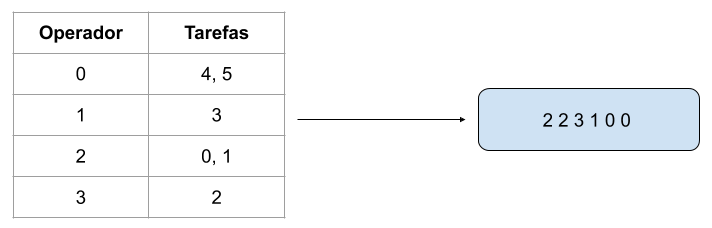
\includegraphics[scale=0.35]{figure1}
\end{figure}

\subsection{População Inicial}
\quad A população inicial é gerada aleatoriamente. Primeiro criam-se $\mu$ permutações e depois $\mu$ partições. Por último, associa-se a cada permutação uma partição, também de forma aleatória. A tabela abaixo ilustra o processo considerando uma instância de 8 tarefas e 4 operadores.
\begin{table}[!]
\centering
\begin{tabular}{ccc}
\hline
\textbf{Permutação} & \textbf{Partição} & \textbf{Indivíduo Gerado} \\ \hline
(0 3 2 1) & 0 0 1 1 2 2 3 3 & 0 0 3 3 2 2 1 1 \\ \hline
(2 3 0 1) & 0 1 1 1 2 3 3 3 & 2 3 3 3 0 1 1 1 \\ \hline
(3 1 0 2) & 0 0 0 0 0 1 2 3 & 3 1 0 0 0 0 0 2 \\ \hline
(1 2 3 0) & 0 1 2 2 2 3 3 3 & 1 2 2 2 3 3 3 0 \\ \hline
\end{tabular}
\end{table}
\newpage
\subsection{Seleção de Indivíduos para Crossover}
\quad A seleção de indivíduos para crossover implica na realização de $\lambda$ $k$-torneios aleatórios. Um $k$-torneio aleatório consiste em selecionar $k$ indivíduos da população de forma aleatória e escolher o melhor desses $k$ indivíduos. 
\subsection{Crossover}
\quad O processo de crossover consiste em criar duas novas soluções usando a partição/permutação de um pai com a partição/permutação do outro. A figura abaixo ilustra o processo. O indivíduo 3 herda a permutação do indivíduo 2 (1 0 2 3)  e a partição do indivíduo 1 (um 0, três 1's, três 2's e três 3's). Já o indivíduo 4 herda a permutação do indivíduo 1 (3 1 2 0) e a partição do indivíduo 2 (dois 0's, três 1's , três 2's e dois 3's).
\begin{figure}[tph!]
\centering
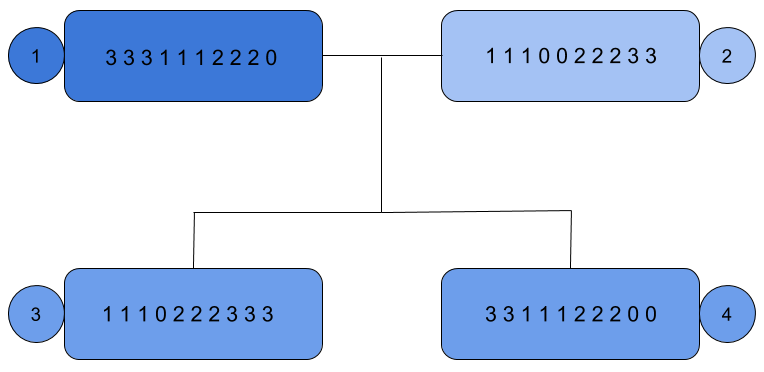
\includegraphics[scale=0.35]{figure2}
\end{figure}
\subsection{Mutação}
\quad O processo de mutação consiste em aplicar uma pequena perturbação aleatória na permutação da solução. A figura abaixo ilustra o processo.
\begin{figure}[tph!]
\centering
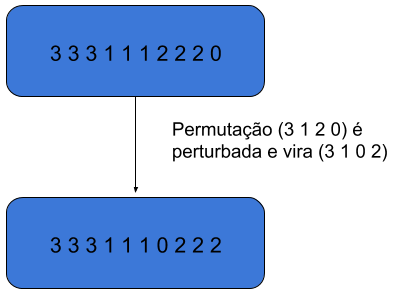
\includegraphics[scale=0.35]{figure3}
\end{figure}
\subsection{Seleção da Nova População}
\quad A seleção da nova população depende do parâmetro $\lambda$ . Se $\lambda$ novos indivíduos foram criados via crossover, então os $\lambda$ piores indivíduos  entre todos os indivíduos (geração atual e nova geração) são eliminados da população.
\subsection{Critério de Parada}
\quad A execução do algoritmo para e retorna uma solução se uma ou mais das condições abaixo forem satisfeitas:
\begin{itemize}
\item O tempo de execução do algoritmo atingiu a marca dos 30 minutos
\item $\omega$ gerações foram geradas e o valor da função objetivo não diminuiu
\end{itemize}



\end{document}

